\documentclass[11pt,a4paper]{article}
\usepackage[utf8]{inputenc}
\usepackage[spanish,es-tabla]{babel}
\usepackage{amsmath}
\usepackage{amsfonts}
\usepackage{amssymb}
\usepackage{graphicx}
\usepackage{natbib}
\usepackage{lineno}
\usepackage{ragged2e}
\usepackage{multicol}
\setlength\columnsep{38pt}
\usepackage{enumerate} 
\usepackage[left=2.8cm,top=2.3cm,right=2.8cm,bottom=2.3cm]{geometry} 
\usepackage{fancyhdr}
\usepackage{url}


\begin{document}
		
		\begin{center}
			\huge \textbf{Aprendizaje Supervisado y No Supervisado} 
		\end{center}
		
		\begin{center}
			
\includegraphics[scale=0.50]{./Imagenes/logo}
		\end{center}
		
		\begin{multicols}{2}
			\small
			\begin{center}
				Marlon Villegas Arando\\
				2015053890\\
				UPT – Ingeniería de Sistemas\\
				EPIS\\
				Tacna, Perú\\
				
				\vspace{\baselineskip}
				Lisbeth Espinoza Caso\\
				2011040667\\
				UPT – Ingeniería de Sistemas\\  
				EPIS\\	
				Tacna, Perú\\                 

			\end{center}
			\normalsize			
		\end{multicols}
		\vspace{\baselineskip}

		\textbf{\textit{\large Resumen}}\rule[1.5mm]{5mm}{0.1mm}	\vspace{\baselineskip}
		
		\\La inteligencia, en pleno siglo XXI, trasciende las fronteras de la mente. Mucho escuchamos decir que ahora los computadores son más inteligentes que los cerebros y que pronto los robots sustituirán a los humanos para pasar a dominar el mundo.\\
		
        \\Está muy arraigada la creencia de que por más inteligente que pueda ser un computador, nunca podrá tener la capacidad de pensar. Sin ánimos de fatalismo, el aprendizaje automático ha revolucionado de forma decisiva el campo de la computación, facilitando la realización de todo tipo de tareas de forma digital y no manual.\\ 
        
        \\El aprendizaje automático, también conocido en inglés como machine learning, es un campo de la computación que lleva a otro nivel a la inteligencia artificial: hace que las computadoras aprendan a pensar.\\
        
        \\No tan literal. Los computadores no desarrollaron un cerebro y ahora tienen emociones. Simplemente el machine learning desarrolla algoritmos que hacen que las máquinas puedan aprender por su cuenta y responder a determinadas preguntas con bastante certeza. Para desarrollar estos algoritmos, existen dos modalidades: aprendizaje supervisado y no supervisado.\\
		
		\newpage
		
		\textbf{\textit{\large Abstract}}\rule[1.5mm]{5mm}{0.1mm} 		
		\textit{	
		 }\vspace{\baselineskip}
		 \\The intelligence, in the 21st century, transcends the frontiers of the mind. We hear a lot to say that computers are now smarter than brains and that soon robots will replace humans to dominate the world.\\
		 
		 \\The belief that as intelligent as a computer may be, it can never have the ability to think is deeply rooted. Without the spirit of fatalism, machine learning has revolutionized the field of computing decisively, making it easier to perform all kinds of tasks digitally and not manually.\\
		 
		 \\Machine learning, also known in English as machine learning, is a field of computing that takes artificial intelligence to another level: it makes computers learn to think\\
		 
		 \\Not so literal. Computers did not develop a brain and now have emotions. Machine learning simply develops algorithms that allow machines to learn on their own and answer certain questions with certainty. To develop these algorithms, there are two modalities: supervised and unsupervised learning.\\
				
		\vspace{\baselineskip}
					
		\rule{167mm}{0.1mm}
		
		\vspace{\baselineskip}
		
		\section{Introduccion}
		
		El aprendizaje automático o machine learning se encuadra como una disciplina de la inteligencia artificial.\\

        El principal objetivo que busca es crear sistemas que sean capaces de aprender automáticamente, es decir que sean capaces de encontrar patrones complejos en grandes conjuntos de datos por si solos.\\

        Los algoritmos de machine learning se suelen clasificar en dos grupos, por un lado se encuentran los algoritmos supervisados que aplican lo que se ha aprendido con los datos históricos para sacar conclusiones sobre nuevos datos y por otro lado se encuentran los algoritmos no supervisados pueden extraer inferencias de conjuntos de datos, aunque existen otros tipos como aprendizaje semi-supervisado, aprendizaje por refuerzo, aprendizaje multi-tarea y transducción.\\
		
		\begin{center}
		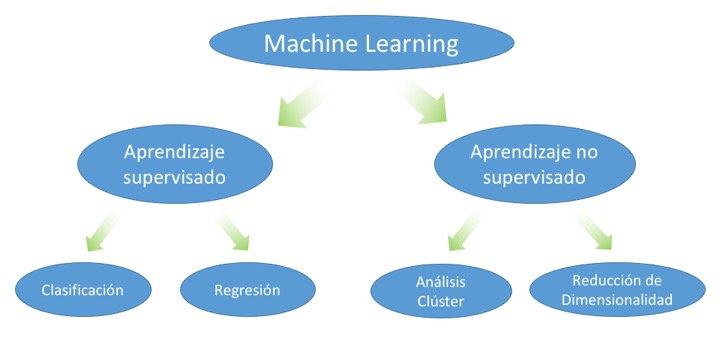
\includegraphics[scale=0.5]{./Imagenes/MachineLearning}
		\end{center}
		
		\section{Aprendizaje Supervisado}
		
			El aprendizaje supervisado es el más común utilizado entre los dos , incluye algoritmos tales como regresión lineal y logístico, clasificación de clases múltiples y máquinas de vectores de soporte.\\

            El aprendizaje supervisado se llama así porque el desarrollador actúa como una guía para enseñar al algoritmo las conclusiones a las que debe llegar, es decir la salida del algoritmo ya es conocida. Es similar a la forma en que un niño podría aprender de un maestro.\\

            Requiere que los posibles resultados del algoritmo ya sean conocidos y que los datos utilizados para entrenar el algoritmo ya estén etiquetados con las respuestas correctas. Por ejemplo, un algoritmo de clasificación aprenderá a identificar animales después de haber sido entrenados en un conjunto de datos de imágenes que están apropiadamente etiquetados con las especies del animal y algunas características de identificación.\\
            
            \begin{center}
		    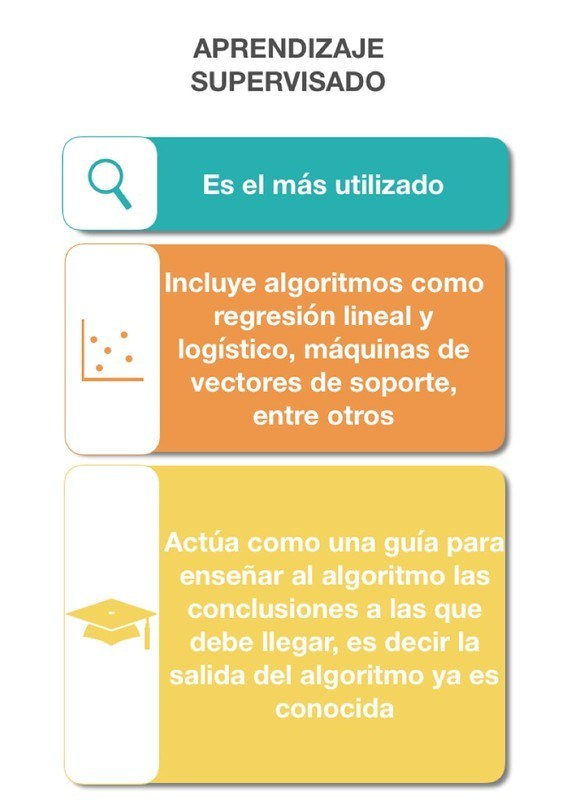
\includegraphics[scale=1.0]{./Imagenes/AprendisajeSupervisado}
		    \end{center}
			
			\subsection{Funciones y Tipos}
			\\La primera modalidad de aprendizaje que tiene el machine learning es la de aprendizaje supervisado. Usándola, se entrena al algoritmo otorgándole las preguntas, denominadas características, y las respuestas, denominadas etiquetas. Esto se hace con la finalidad de que el algoritmo las combine y pueda hacer predicciones.\\
            
            \\Existen, a su vez, dos tipos de aprendizaje supervisado:\\
		
			\begin{enumerate}[A.]
			
			\item Regresión:
			
			    Tiene como resultado un número específico. Si las etiquetas suelen ser un valor numérico, mediante las variables de las características, se pueden obtener dígitos como dato resultante.\\
			
			    \begin{center}	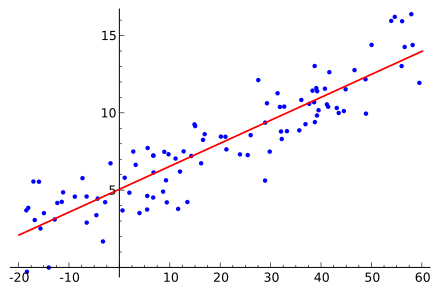
\includegraphics[scale=0.5]{./Imagenes/regresion}
    			\end{center}
			
			    \\Donde se predice un valor real basado en entradas pasadas. Estos algoritmos se usan para predecir valores de salida basados en algunas características de entrada obtenidas de los datos. A esto, el algoritmo construye un modelo basado en las características y los valores de salida de los datos de entrenamiento y este modelo se usa para predecir los valores para nuevos datos. Los valores de salida en este caso son continuos y no discretos.\\

                \\Algunos ejemplos de este algoritmo son: predecir los precios de la vivienda, predecir las cantidades de compra, predecir la cantidad de ingresos se genera a partir de una nueva campaña de marketing.\\
                
                \\Los tipos de algoritmos de regresión incluyen:\\
                
                \begin{itemize}
			    \item Regresión lineal
			    \item Regresión polinomeal
			    \item Vectores de soporte regresión
			    \item Arboles de decisión regresión
			    \item Bosques aleatorios regresión
		        \end{itemize}
                
                \begin{center}
		        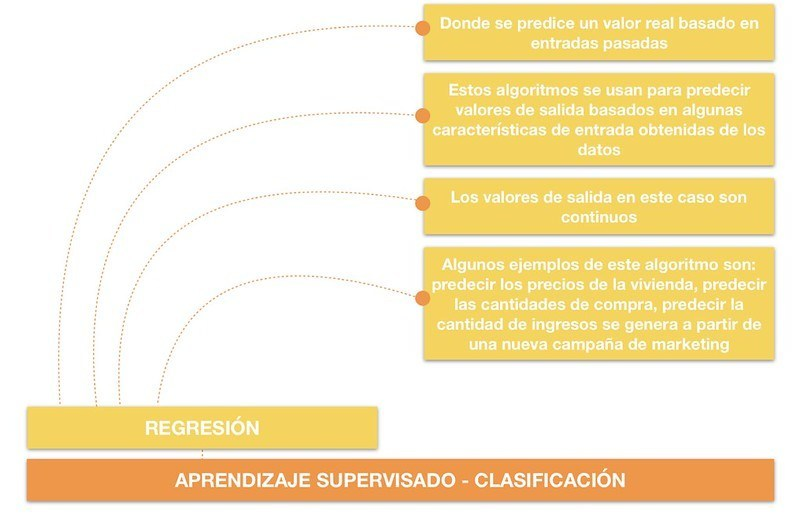
\includegraphics[scale=1.0]{./Imagenes/AprendSuperRegresion}
		        \end{center}

    		\item Clasificación: 
    		    
    		    \\En este tipo, el algoritmo encuentra diferentes patrones y tiene por objetivo clasificar los elementos en diferentes grupos.\\
			
    			\begin{center}	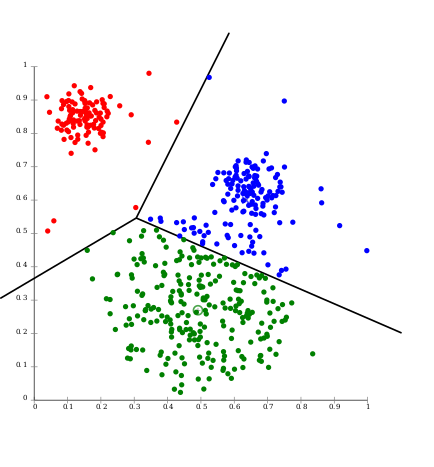
\includegraphics[scale=0.5]{./Imagenes/clasificacion}
    			\end{center}
			
			    \\El algoritmo no está en capacidad de determinar a qué grupo pertenece un valor o cuál es el resultado de una operación. Solamente logra relacionar características con etiquetas y así obtener un resultado.\\
			    
			    \\El algoritmo intenta etiquetar cada ejemplo eligiendo entre dos o más clases diferentes. Estos algoritmos crean modelos predictivos a partir de datos de capacitación que tienen características y etiquetas de clase.\\
			    
			    \\Estos modelos predictivos, a su vez usan las características aprendidas de los datos de capacitación sobre datos nuevos, no vistos previamente, para predecir sus etiquetas de clase. Elegir entre dos clases se denomina clasificación binaria, como predecir si alguien incumplirá un préstamo. Elegir entre más de dos clases se denomina clasificación multiclase.\\

                \\Algunos ejemplos de este algoritmo son: predecir si un cliente va a cancelar o no su tarjeta de crédito, predecir si un alumno pasará o no una clase.\\

                \\Los tipos de algoritmos de clasificación incluyen:\\

                \begin{itemize}
			    \item Regresión logística
			    \item Vecinos más cercanos
			    \item Máquinas de vectores de soportes
			    \item Arboles de decisión clasificación
			    \item Bosques aleatorios clasificación
		        \end{itemize}
                
                \begin{center}
		        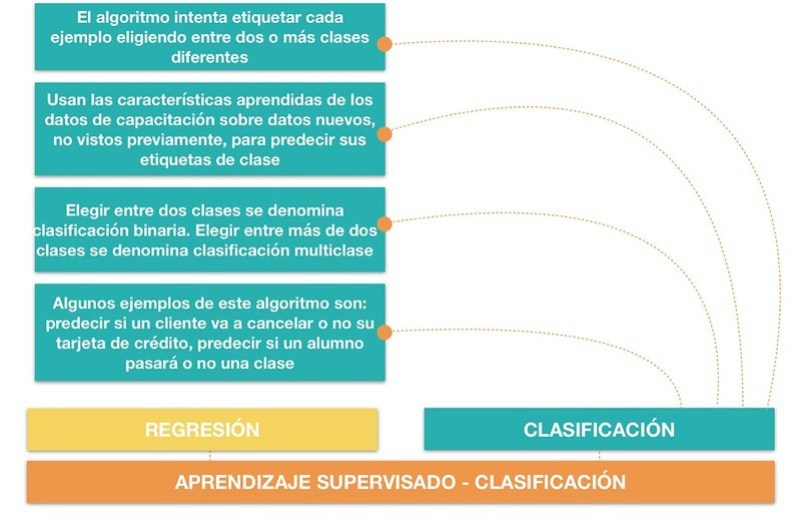
\includegraphics[scale=1.0]{./Imagenes/AprendSuperClasificacion}
		        \end{center}
			
			\end{enumerate}
			
		    \\En el aprendizaje supervisado, los algoritmos trabajan con datos “etiquetados” (labeled data), intentado encontrar una función que, dadas las variables de entrada (input data), les asigne la etiqueta de salida adecuada. El algoritmo se entrena con un “histórico” de datos y así “aprende” a asignar la etiqueta de salida adecuada a un nuevo valor, es decir, predice el valor da salida.\\

            \\Por ejemplo, un detector de spam, analiza el histórico de mensajes, viendo qué función puede representar, según los parámetros de entrada que se definan (el remitente, si el destinatario es individual o parte de una lista, si el asunto contiene determinados términos etc), la asignación de la etiqueta “spam” o “no es spam”. Una vez definida esta función, al introducir un nuevo mensaje no etiquetado, el algoritmo es capaz de asignarle la etiqueta correcta.\\

            \\El aprendizaje supervisado se suele usar en problemas de clasificación, como identificación de dígitos, diagnósticos, o detección de fraude de identidad.  También se usa en problemas de regresión, como predicciones meteorológicas, de expectativa de vida, de crecimiento etc. Estos dos tipos principales de aprendizaje supervisado, clasificación y regresión, se distinguen por el tipo de variable objetivo. En los casos de clasificación, es de tipo categórico, mientras que, en los casos de regresión, la variable objetivo es de tipo numérico.\\
            
            \subsection{Aprendizaje Supervisado en el Machine Learning}
            
            \\El objetivo básico de Machine Learning es utilizar computadoras para obtener información, sin que se indique explícitamente que lo haga. En la mayoría de los casos esto implica utilizar un conjunto de resultados históricos para hacer predicciones sobre los resultados futuros.\\ 
            
            \\Esto se vuelve útil cuando se quiere automatizar las percepciones sobre conjuntos de datos de gran tamaño, lo que sería demasiado difícil de realizar para un ser humano de manera recurrente.\\
            
            \begin{center}	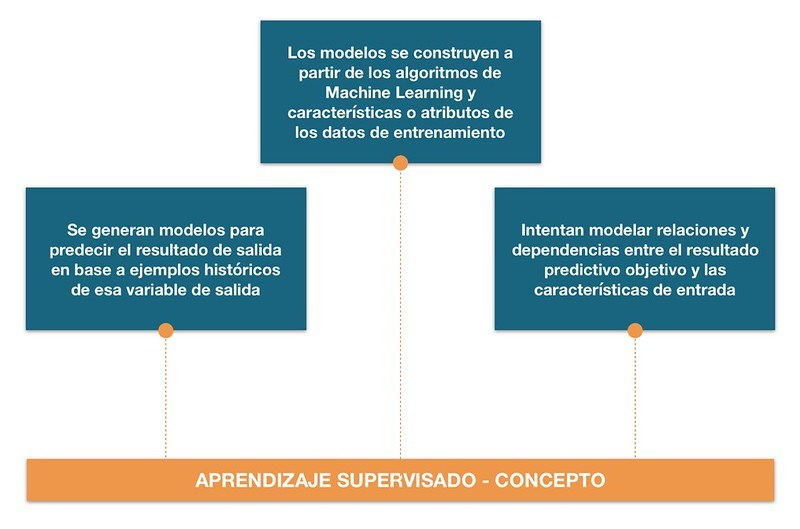
\includegraphics[scale=1.0]{./Imagenes/AprendizajeSupervisadoConcepto}
    		\end{center}
    		
    		\\Por su parte, el aprendizaje supervisado se refiere al subconjunto de Machine Learning donde se generan modelos para predecir el resultado de salida en base a ejemplos históricos de esa variable de salida.\\ 
    		
    		\\Los modelos se construyen a partir de los algoritmos de Machine Learning y características o atributos de los datos de entrenamiento para que podamos predecir el valor utilizando otros valores obtenidos a partir de datos de entrada.\\

            \\Los algoritmos de aprendizaje supervisado intentan modelar relaciones y dependencias entre el resultado predictivo objetivo y las características de entrada para que podamos predecir los valores de salida para datos nuevos en función de las relaciones que aprendió de los conjuntos de datos anteriores.\\
            
            \subsection{Importancia del aprendizaje supervisado}
            
            \\El aprendizaje supervisado proporciona una ruta directa para convertir datos en información real y procesable. Al utilizar los datos como un recurso, les permite a las organizaciones comprender y prevenir los resultados no deseados o impulsar los resultados deseados para lo que sea que estén tratando de predecir.\\

            \\Por ejemplo, pueden decirle a una empresa que los clientes presentan un alto riesgo de agitación, la compañía puede llegar a ese cliente en particular con comunicaciones dirigidas y ofertas promocionales, lo que reduce su predisposición al abandono.\\

            \\Este aprendizaje es uno de los motores más potentes que permite que los sistemas de inteligencia artificial tomen decisiones empresariales de forma más rápida y precisa que los humanos.\\

            \\Sin embargo, la implementación exitosa de algoritmos de aprendizaje supervisado ha requerido gran cantidad de tiempo y la experiencia técnica de equipos especializados con el fin de construir, escalar y desplegar modelos predictivos precisos. Además, dado que los modelos de aprendizaje supervisado hacen predicciones del mundo real basado en los datos del pasado, los modelos deben ser reconstruidos periódicamente con el fin de mantener sus predicciones sin que se conviertan en obsoletas ya que en ocasiones el comportamiento de los datos puede cambiar.\\
            
            \begin{center}	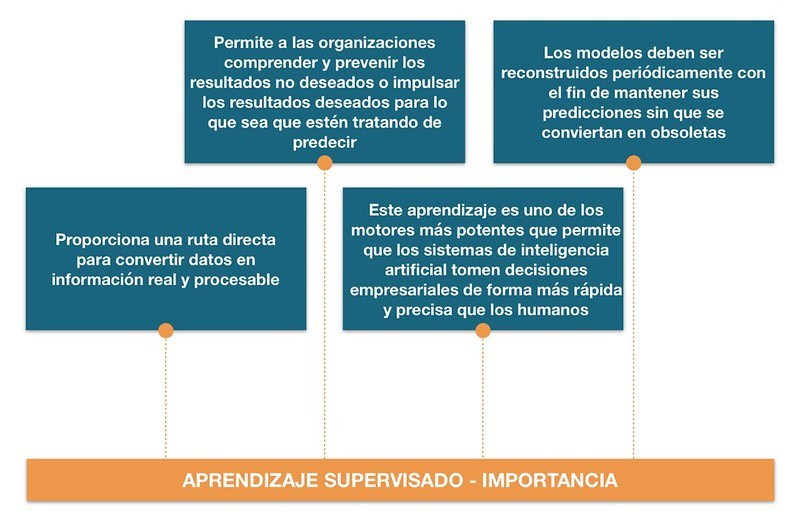
\includegraphics[scale=1.0]{./Imagenes/AprendSuperImportancia}
    		\end{center}
    		
    		\\En conclusión, el aprendizaje supervisado aprende de datos etiquetados, es decir, los datos del cual conoce la variable resultado, y hace predicciones para ese resultado en nuevos conjuntos de datos. Es importante tener en cuenta que solo funciona si su conjunto de datos históricos contiene valores reales para el resultado que intenta predecir.\\

	        \subsection{Algoritmos de Clasificación}
	        
	        \begin{enumerate}[A.]
		
			\item \textbf{Regresión Logística:}
			
			\\Uno de los principales problemas en la clasificación ocurre cuando el algoritmo nunca converge en la actualización de los pesos mientras está siendo entrenado.\\
            
            \\Esto ocurre cuando las clases no son perfectamente separables linealmente. Por tanto, para tratar con problemas de clasificación binaria la regresión logística es uno de los algoritmos más usados.\\
            
            \\La regresión logística es un algoritmo de clasificación (a pesar de su nombre) simple, pero potente . Funciona muy bien en clases linealmente separables y se puede extender a clasificación multiclase , a través de la técnica OvR.\\
			
			\item \textbf{Máquinas de Vector Soporte (SVM):}
			
			\\Este algoritmo puede ser considerado una extensión del algoritmo “perceptron”. En SVM el objetivo de la optimización es establecer una línea de decisión que separe las clases maximizando el margen entre esta línea y los puntos de muestra cercanos a este hiperplano. Estos puntos se llaman vectores soporte.\\
			
			\begin{center}
		    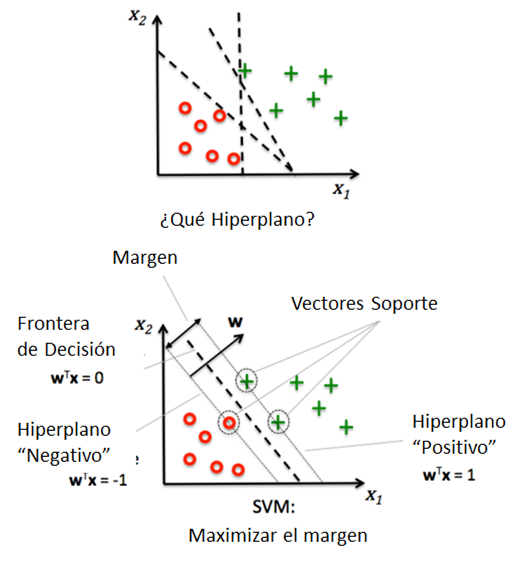
\includegraphics[scale=0.7]{./Imagenes/SVM}
		    \end{center}

			\end{enumerate}
	    
\end{document}		
